\documentclass{article}
\usepackage[utf8]{inputenc}
\usepackage{graphicx} % Required for including images
\usepackage{amsmath, amssymb} % Required for math features
\usepackage{hyperref} % For hyperlinks
\usepackage{natbib} % For bibliography
\usepackage{geometry} % For page dimensions and margins
\geometry{a4paper, margin=1.2in}

\title{Machine Learning Project Report: Neural Network Implementation on MNIST Dataset}
\author{Noé Bourgeois}
\date{Academic Year 2023-2024}

\begin{document}

\maketitle

\begin{abstract}
% Write your abstract here
\end{abstract}

\section{Introduction}
% Introduce the project, its objectives, and significance

% \section{Methodology}
\section{Experimentation Framework}
% Describe the methodology, including neural network architecture, 
% forward propagation, error calculation, and backpropagation

\subsection{Neural Network Architecture}
% Details about the neural network layers, activation functions, etc.

\subsection{Forward Propagation}
% Explain the forward propagation process

\subsection{Error Calculation}
% Describe how the error is calculated (mean squared error, etc.)

\subsection{Backpropagation}
% Explain the backpropagation process for weight updates

\section{Results}
% Present the results of your experiments
% Include graphs, tables, and confusion matrix visualizations
\subsection{Training}
\subsection{Testing}
\subsubsection{Confusion Matrix}
% graph:
\begin{figure}
% \begin{figure}[h] % h forces the figure to be placed here
% \begin{figure}[h!] % ! after h forces the figure to be placed here
    \centering
    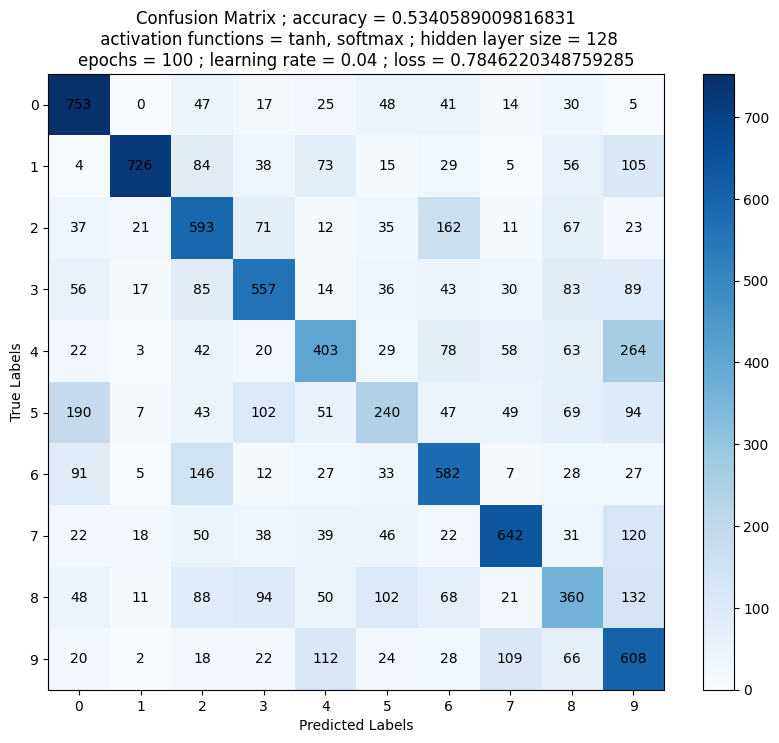
\includegraphics[width=\textwidth]{media/confusion/confusion_matrix_activation_functions_tanh_softmax_hidden_layer_size_128_epochs_100_learning_rate_0.04_loss_0.7846220348759285.png}
    \caption{Confusion Matrix for tanh activation function, softmax output function, 1 hidden layer of 128 neurons, 100 epochs, 0.04 learning rate, and 0.7846220348759285 loss.}
    \label{fig:confusion}
\end{figure}
\subsubsection{Accuracy}
\subsubsection{Prediction}
\begin{figure}
    \centering
    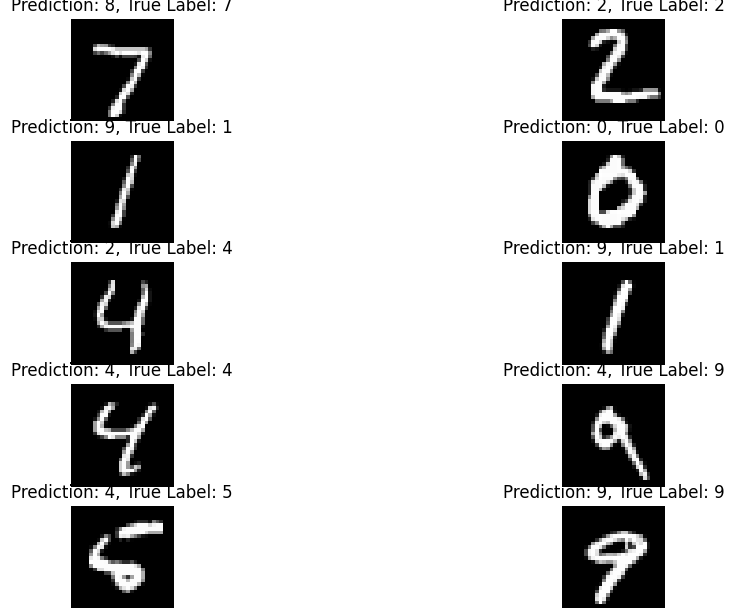
\includegraphics[width=\textwidth]{media/prediction/4.png}
    \caption{Prediction}
    \label{fig:Prediction}
\end{figure}
\subsection{Convolution}
98.8\% accuracy
\subsubsection{Confusion Matrix}
% graph:
\begin{figure}
    \centering
    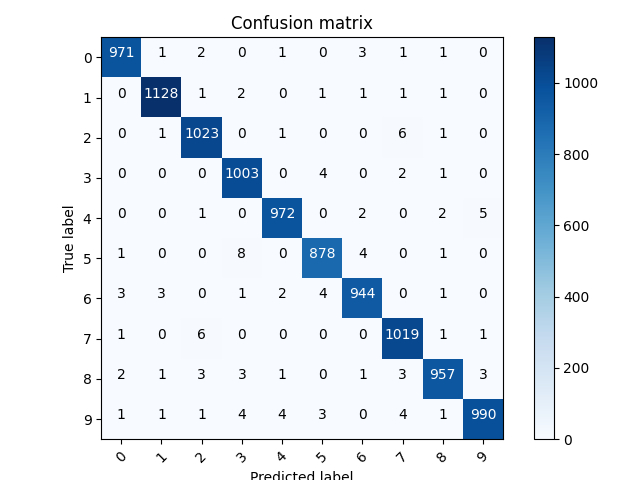
\includegraphics[width=\textwidth]{media/convolution/Figure_1.png}
    \caption{Confusion Matrix for convolutional model.}
    \label{fig:convolution_confusion}
\end{figure}

% \section{Discussion}
\section{Analysis}
% Discuss the results, what they mean, and any conclusions you can draw

\section{Conclusion}
% Summarize the main findings and future work
\subsection{Main Findings}
\subsection{Tools}
\subsubsection{Assistance}
\begin{itemize}
    \item ChatGPT
\end{itemize}
\subsection{Future Work}
\section{References}
% Include your references here
\bibliographystyle{plain}
\bibliography{references} % references.bib should be the name of your BibTeX file

\end{document}
